\chapter{Einleitung}

\anno{ca. 5 Seiten}

\begin{neu}
  Lässt sich hier eine Einleitung aus den drei vorherigen Papers ableiten? ggf. Master Expose mit hinzuziehen!
\end{neu}

Jeder Betreiber von Anwendungen im Internet, vom kleinen Blog bis zur großen Geschäftsanwendung, ist auch dem Risiko ausgesetzt dass potentielle Angreifer versuchen werden den Betrieb zu stören oder zu manipulieren. Der Schutz von Anwendungen im Bereich IT-Sicherheit ist daher eine Notwendigkeit, gehört aber meistens nicht zum Kerngeschäft dieser Nutzer. Größtenteils wird sich dann darauf verlassen dass die betriebene Anwendung gegen alle möglichen Angriffsmöglichkeiten gewappnet ist. Bei der Anforderungsanalyse sehen die fachlichen Nutzern die Umsetzung ihrer Geschäftsprozesse im Vordergrund. In vielen Fällen wird peinlichst genau definiert wo ein Eingabefeld zu stehen hat oder in welcher Form und Farbe ein Bestätigungknopf darzustellen ist. Beim Thema Sicherheit heißt es jedoch häufig \glqq\emph{Die Anwendung muss sicher sein.}\grqq \\
Letztendlich muss man das Rad auch nicht neu erfinden und auch die Hersteller von Software sind froh wenn für allgemeine Probleme einfache, wiederverwendbare Lösungen genutzt werden können. \\\\
\anno{Ziel der Arbeit}
Eine \emph{einfache}, \emph{wiederverwendbare} Lösung im Bereich der IT-Sicherheit von webbasierten Anwendungen sind sogenannte \emph{Web Application Firewalls} (WAF). Im einfachsten Fall sitzen diese Systeme zwischen Endanwendern und der zu schützenden Anwendung, belauschen den Datenverkehr und filtern jegliche schädliche Kommunikation. Je besser eine WAF die zu schützenden Anwendungen kennt desto einfacher fällt ihr die Unterscheidung zwischen \emph{schädlichem} und \emph{nicht-schädlichem} Datenverkehr. Häufig ist die Konfiguration jedoch sehr umfangreich und komplex. Ziel dieser Arbeit ist das Aufzeigen einer möglichen Vereinfachung der Konfiguration in der Praxis. Mehrere Systeme bzw. schützende Anwendungen werden durch einen zentralen Bestandteil miteinander verbunden und können so gegenseitig von einander lernen.\\\\

\anno{Methodik 1 Seite }
Im Laufe der Arbeit wird exemplarisch ein Prototyp mit Testumgebung entwickelt \anno{experimentell} und anschließend unter Zuhilfenahme ausgewählter \anno{Stichprobe} Anwendungen und Angriffsmuster getestet. Für den Test müssen in einem ersten Schritt mögliche Anwendungen als Testkandidaten anhand qualitativer Kriterien (Ähnlichkeit) ausgewählt werden. Für einen späteren Vergleich werden bei  einem Test mit reproduzierbarem Angriffsmuster aber ohne Firewall Kennzahlen ermittelt. Diese können später mit den Kennzahlen aus dem reproduzierten Test, dann mit aktivierter Web Application Firewall, verglichen werden. Funktionalität und Effektivität werden im Anschluss bewertet. 

Jährlich erscheint mit den OWASP Top Ten \cite{owasp10}  eine Liste der meist genutzten und bekannten Sicherheitsrisiken für Webanwendungen. In den meisten Fällen wird eine Anwendung sehr indiviuell gegen solche Risiken abgesichert und häufig wird dabei auch jedes einzelne Risiko separat adressiert. WebApplicationFirewalls (WAF) bieten einen relativ einfachen Weg einen Großteil der Risiken allgemein auszuschließen. Die Konfiguration einer WebApplicationFirewall muß jedoch auf die jeweilig zu schützende Anwendung angepasst werden. Mit dieser Masterarbeit soll eine Möglichkeit zur einfacheren Einbindung dieser Schutzmaßnahme bereitgestellt werden. Es wird gezeigt wie eine ältere WAF-Software auf einen neuen Stand gebracht wird und mehrere Instanzen dieser Software gekoppelt werden können. Mittels selbständiger Kategorisierung wird dem Nutzer die individuelle Konfiguration abgenommen und ein messbarer Gewinn an Sicherheit für viele Anwendungen bereitgestellt. \anno{aus Exposee übernommen}


\begin{figure}[bht]
  \begin{center}
    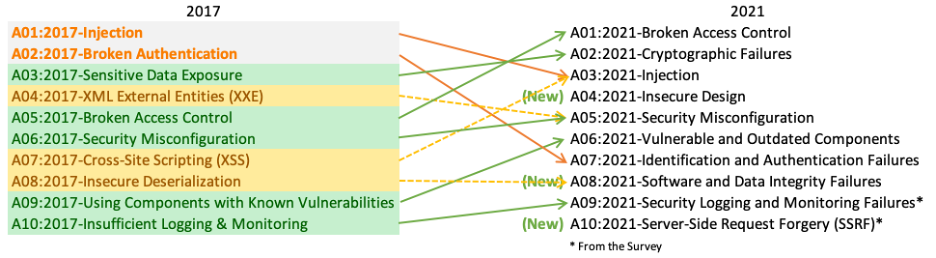
\includegraphics[width=15cm]{mapping}
    \caption{OWASP Top10 2017/2021 \cite{owasp10}}
    \label{fig.topten}
  \end{center}
\end{figure}

% das grosse Problem
%% Was ist der Markt
%%% zahlreiche Anbieter teils spezialisiert auf bestimmte Bereiche; zahlreiche Arten von WAF
%% Wem hilft es?
%% Warum jetzt?
%% Ist das Problem lösbarer geworden?

\section{Zielsetzung}
% Ziel der Arbeit
%% Was ist Ihr relevantes Teilproblem? Was ist die zentrale Frage?
%% Ihr Ziel in zwei Absätzen.
%%% Warum genau dieses Problem?
%%% Ist Ihr Beitrag völlig neu, oder nur ein Baustein?
%%% Ist Ihr Proble schwer zu lösen oder straight forward?
%%% Eher Forschung oder Anwendung?
%%% Was machen Sie nicht? Und warum haben Sie sich entschieden das nicht zu machen.
%% Wenn Sie ein System bauen...
%%% Welche Anfragen/Aufgaben wollen Sie beantworten/lösen können?
%%% Welche Kernfunktionalität soll Ihr System haben?
%%% Was ist ein typischer (Bedienungs-)Prozess für Ihr System



% Methodik (1 Seite)
%% Wie wollen Sie das Problem lösen?
%% Welche Grundlagen müssen Sie beachten?
%% Wie ist Ihre Vorgehensweise?

% Gliederung und Aufbau (ca. 0,5 Seiten)
%% Wann lesen wir was und warum?
\section{Aufbau der Arbeit}

% erster Teile Grundbegriffe, verwandte Vorarbeiten und

Dieses \textbf{erste Kapitel} der Arbeit lieferte bereits einen kurzen Einblick in die Thematik. Das folgendende \textbf{zweite Kapitel} erläutert noch wichtige Grundbegriffe aus den Bereichen der IT-Sicherheit die zum Verständnis der Thematik beitragen, gefolgt von einer kurzen zeitlichen Einordnung zur Entwicklung der Web Application Firewalls in den letzten Jahren. Das folgende, dritte Kapitel enthält die Kernelemente der Arbeit und schlägt mögliche Verbesserungen vor. Der derzeitige Stand wird genauer betrachtet und mögliche Probleme mit Vorschlägen zu deren Lösung aufgezeigt. \textbf{Kapitel 4} gibt einen kurzen Einblick über stattgefundene Arbeiten zur technischen Umsetzung der Vorschläge aus dem vorhergehenden Kapitel . Im anschließenden Kaptitel findet in einer kurzen Demonstration die Auswertung statt und die Arbeit schließt mit einem kurzen Ausblick ab.

\section{Abgrenzung}

Diese Arbeit beschäftigt sich mit der Erweiterung eines bereits bestehenden Produktes und soll anhand praktischer Beispiele Möglichkeiten zur Verbesserung aufzeigen. Die in der Arbeit erwähnten Konzepte und Strategien lassen sich sicherlich auch auf andere Produkte übertragen, dieses soll jedoch nicht Inhalt in dieser Arbeit sein.
